\chapter{Alcance y objetivos}\label{cha:alcance}
La mejora en la miniaturización de la tecnología y la calidad de los servicios
de comunicación ha llevado a que el concepto de ciudad inteligente sea más
viable que nunca. Este proyecto propone el diseño, desarrollo y validación de
un escenario de movilidad cooperativa, segura y eficiente en la cual los
usuarios (conductores, pasajeros y ciclistas) dispongan de una serie de
aplicaciones, que proporcionen información y reciban información, la cual es
procesada en tiempo real. Son tres los retos que afronta este proyecto:

\begin{enumerate}
	\item Diseñar una infraestructura de comunicaciones dinámica, y que integre
	diferentes tecnologías de comunicaciones de corto (\Gls{802.11p}) y largo
	alcance (\gls{lte}).

	\item Procesar la información generada por todos los usuarios y agentes en la
	infraestructura.

	\item Promover la participación de todos los usuarios.

\end{enumerate}
Para lograrlo, como puede observarse en la Figura \ref{fig:despliegue} este
proyecto combina información centralizada en la nube y tecnologías de
computación distribuida con tecnologías de comunicaciones, donde las
comunicaciones \gls{v2x} y las comunicaciones móviles son utilizadas
indistintamente para proporcionar información relevante a todos los usuarios.
Gracias a ello, este proyecto favorecerá un entorno donde los vehículos,
Smartphone y/o Tablet podrán operar entre ellas para proveer servicios de
movilidad a los usuarios.

Este proyecto, basándose en la arquitectura \gls{its} definida por ITS EN 302
665, integrará información procedente de elementos de infraestructura,
vehículos, terminales móviles con servicios desplegados en la nube y ofrecidos
a los usuarios, en una red colaborativa capaz de diferenciar necesidades
individuales y globales. Para ello, los datos recogidos serán procesados por
algoritmos preparados para procesar grandes volúmenes de información, y que
tendrán en cuenta los efectos globales de sus acciones, para lo cual se
dispondrá de enlace de control para regular los sistemas de un modo
descentralizado. Por tanto, el sistema deberá responder dinámicamente las
necesidades de los usuarios.

Se ha seleccionado la tecnología \gls{lte} ya que se ha establecido como la
siguiente generación de comunicaciones móviles, disponible masivamente y
favorecerá el despliegue de \gls{its}. De este modo, la integración de
tecnologías de corto alcance como \Gls{802.11p} con \gls{lte} es obligatorio
para la rápida adopción de aplicaciones para la movilidad.

Para validar este proyecto, se implementarán las siguientes aplicaciones:
\begin{itemize}
	\item Intersecciones seguras: los vehículos próximos a una intersección
	intercambiarán su destino en la misma, avisando de su presencia para evitar
	accidentes.

	\item Navegación segura: los usuarios vulnerables de la carretera podrán
	reportar su posición a los vehículos que les rodeen y al mismo tiempo ser
	alertados de vehículos que se aproximen.

	\item Conducción colaborativa: se desplegarán una serie de aplicaciones
	destinadas a mejorar la eficiencia de las infraestructuras y su seguridad
	gracias a los datos intercambiados entre todos los usuarios y elementos fijos:
	frenada de emergencia, cambio de carril, velocidad adaptativa, etc.
\end{itemize}

El principal objetivo de este trabajo es el desarrollo de aplicaciones para
hacer posible la comunicación entre vehículos y ciclistas, a través de redes
vehiculares y móviles. Se desea que estos dos agentes de la carretera posean
información para poder conocer la posición relativa de los agentes a su
alrededor y así poder evitar accidentes. Las aplicaciones desarrolladas serán
desplegadas por un lado en los sistemas embarcados de los vehículos y la
infraestructura en la carretera, en los móviles inteligentes de los ciclistas y
en la nube, donde un servidor central permitirá la comunicación entre diferentes
plataformas. Se busca la creación de una plataforma lo más abierta posible a
diferentes tecnologías, así como el uso de software libre para su desarrollo.

La verificación del proyecto se hará a través de las pruebas unitarias que se
han creado para probar el sistema, las pruebas que se han realizado en la calle
y a las conclusiones que se han llegado tras analizar las mediciones obtenidas.
Se desea verificar la calidad de las comunicaciones entre los diferentes agentes
de la carretera, así como la precisión de los algoritmos desarrollados para
prever los accidentes y obtener información a través de los datos recogidos por
los mensajes vehiculares. Para saber más sobre cómo se han verificado los
resultados del proyecto ir al Capítulo \ref{cha:pruebas}.

Las aplicaciones que serán desarrolladas deben poseer una serie de
características:
\begin{itemize}
	\item Universalidad: el sistema a desarrollar debe ser flexible a diferentes
	tecnologías. Actualmente existen diversos fabricantes que aún no cumplen los
	estándares que se están estableciendo, por lo que se debe permitir que la
	adaptación de los diferentes sistemas sea lo más sencillo posible.

	\item Interfaz gráfica: la interacción del usuario con las aplicaciones debe
	ser sencilla, que no requiera de ningún conocimiento técnico para realizar sus
	funciones.

	\item Localización de agentes en carretera: los vehículos y ciclistas
	intercambian información sobre sus posiciones a través de mensajes \gls{cam}.

	\item Predicción de accidentes: los usuarios deben poder percibir las
	situaciones de peligro. En el caso de los vehículos a motor se reproduce una
	alarma sonora, y en el de los ciclistas se enciende un led que llevan colocado
	en el casco, además de mostrarse la alerta en el smartphone; en caso de
	tenerlo a la vista.
\end{itemize}

\begin{figure}[h]
	\begin{center}
			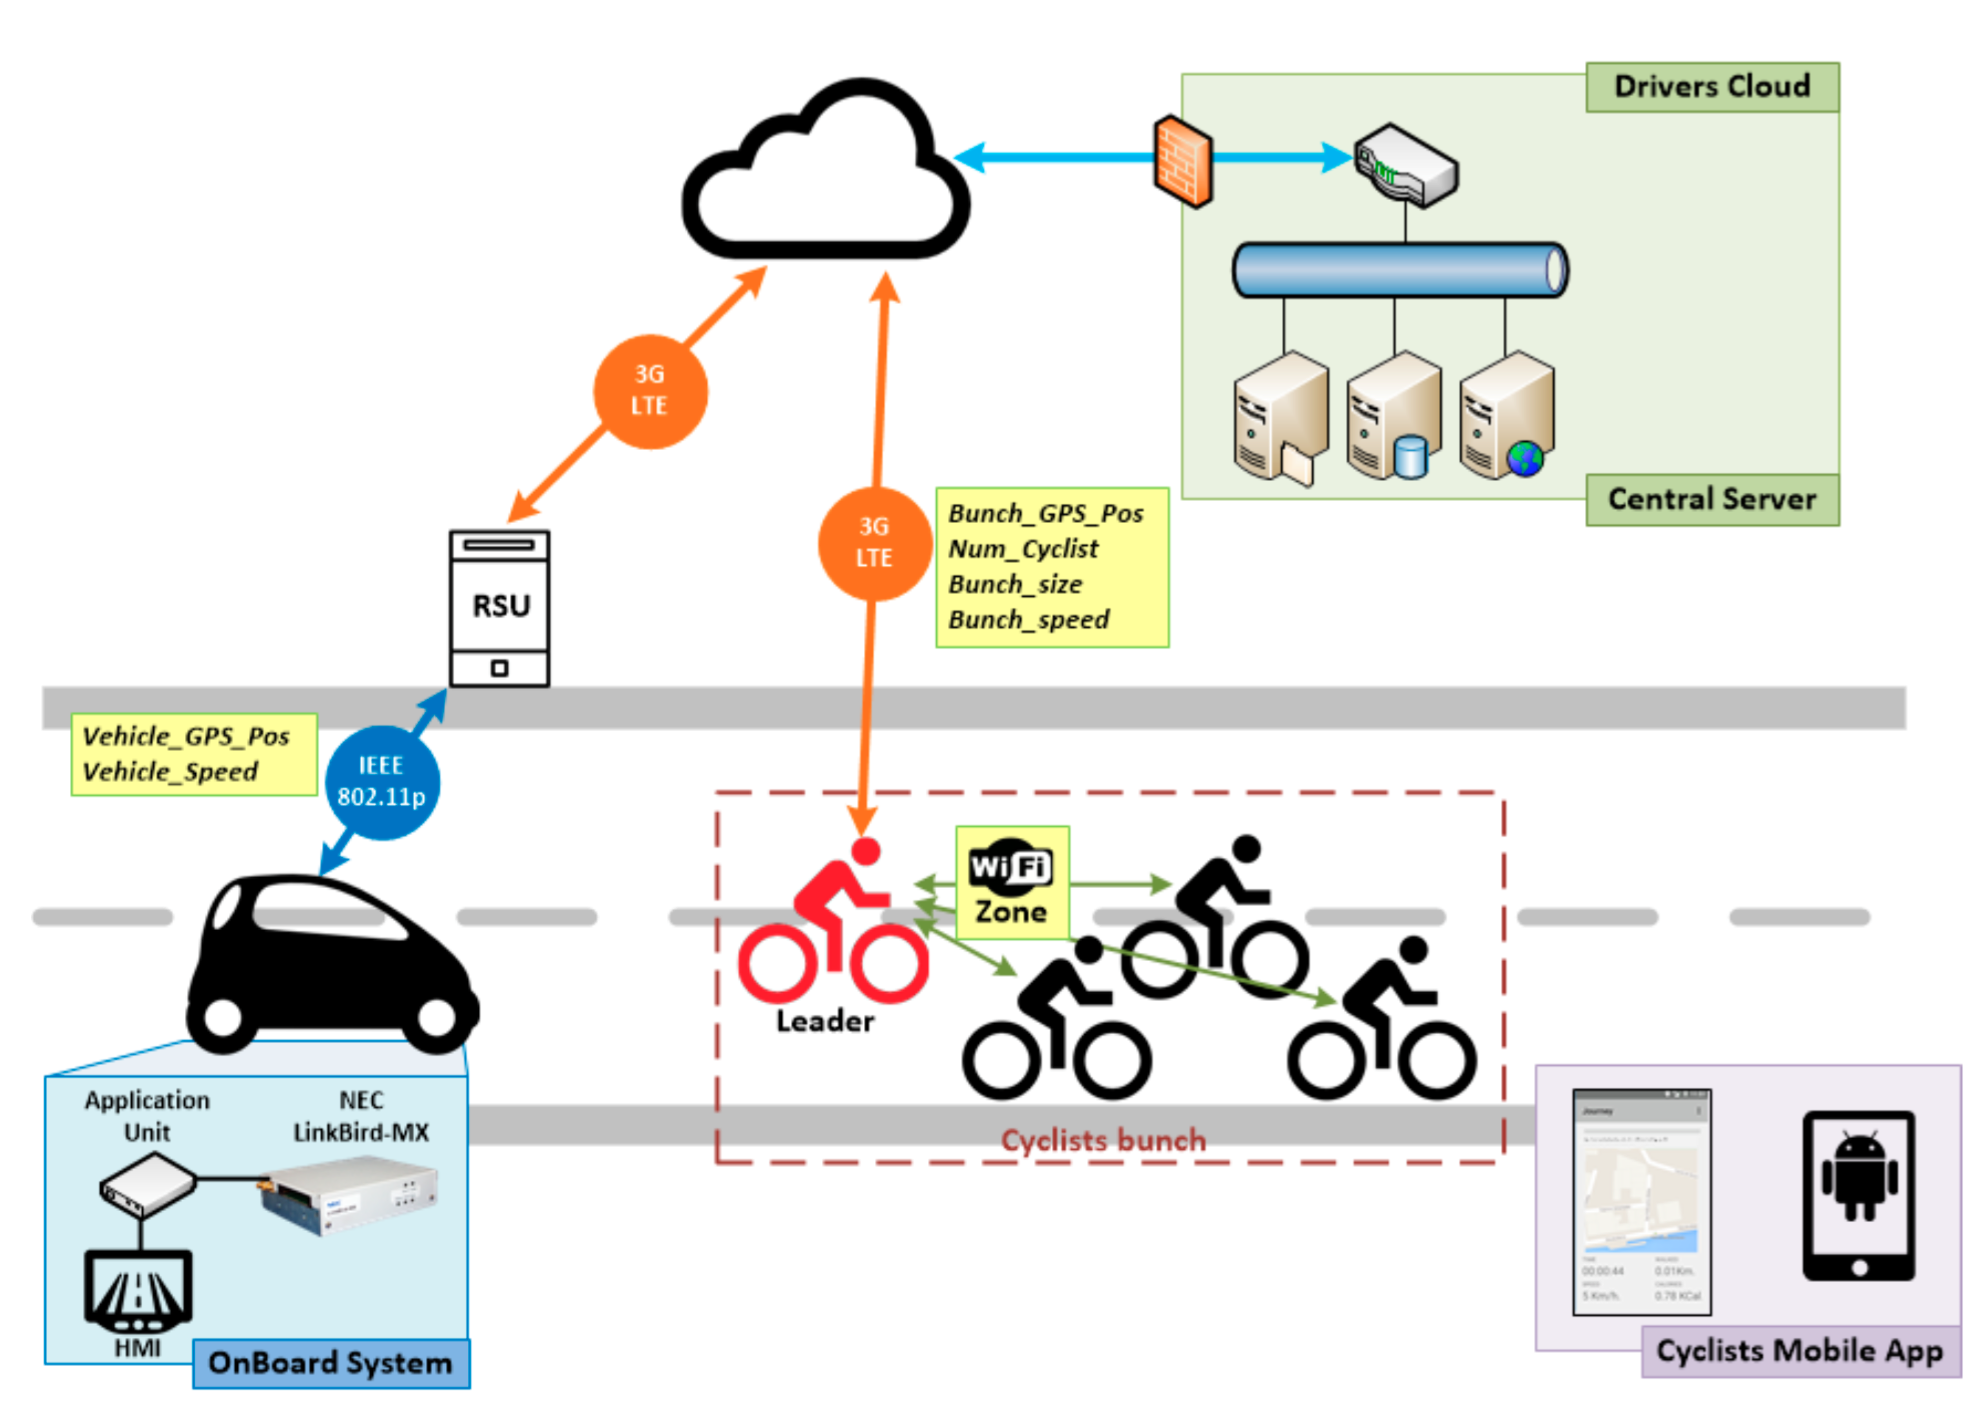
\includegraphics[scale=0.35]{Diag-despliegue}
		\caption{Diagrama de sistema desplegado}
		\label{fig:despliegue}
	\end{center}
\end{figure}

\FloatBarrier
\chapter{Producto final}
El producto final se divide en tres grupos de aplicaciones que están presentes en diferentes agentes de la carretera. Cada grupo de aplicaciones está formado por software y hardware y constituye una unidad desde el punto de vista de usuario.

El primer grupo se trata del sistema en la nube que se encarga de comunicar el lado de vehículos a motor y ciclistas. Además, detecta situaciones de peligro y pone en aviso a cada agente implicado. Estas son las funciones que debe cumplir:
\begin{itemize}
	\item Aplicación web: la nube debe poder accederse a través de una aplicación web, empleando servlets para recibir y procesar la información.
	
	\item Base de datos: se deben poder almacenar datos de las peticiones enviadas por los vehículos. No es necesario que los datos sean persistentes, cuando la aplicación	se cierra los datos deben ser eliminados.
	
	\item Algoritmos para la detección de colisiones: se implantarán algoritmos para detectar la proximidad entre dos vehículos, para actuar en consecuencia.
	
	\item Sistema de avisos: debe poder enviar mensajes a diferentes plataformas a través de redes móviles.
	
	\item Sistema cloud: la aplicación debe estar preparada para ser desplegada y ejecutada en la nube.
\end{itemize}

El segundo grupo se trata de todas las aplicaciones encargadas de obtener información en la red vehicular, y recibir la información generada en la nube: \gls{rsu}, \gls{obu} y \gls{hmi}. Por una parte, el \gls{obu} debe cumplir los siguientes requisitos:
\begin{itemize}
	\item Comunicación vehicular: debe poder comunicarse con otros dispositivos que	componen la red vehicular.
	
	\item Sistema de navegación: debe implementar un sistema de navegación GPS para	poder obtener las posiciones del vehículo en todo momento. Se requiere que estos datos sean altamente precisos.
	
	\item Canal para sincronizar dispositivos: debe ser posible emparejar un dispositivo móvil para mostrar la información obtenida al usuario.
\end{itemize}

Los requisitos que debe cumplir el \gls{hmi} son:
\begin{itemize}
	\item Canal para sincronizar dispositivos: el dispositivo debe poder emparejarse a la infraestructura del vehículo. Preferiblemente se desea que de forma inalámbrica.
	
	\item Universalidad: la aplicación a desarrollar debe ser desplegada al mayor número de usuarios posible.
	
	\item No debe ser una distracción: emplear el menor número de elementos dinámicos posibles, ya que al ser usado durante la conducción no debe distraer al conductor. Emplear forma visual y sonora para notificar al usuario de los eventos en carretera.
\end{itemize}

Por otra parte los requisitos del \gls{rsu} son:
\begin{itemize}
	\item Comunicación vehicular: debe poder comunicarse con otros dispositivos que componen la red vehicular.
	
	\item Comunicación móvil: debe tener acceso a Internet a través de una red móvil.
	
	\item Sistema de retransmisión: debe poder retransmitir los mensajes que recibe de la red de conductores, con la menor latencia posible.
\end{itemize}

Finalmente, el último grupo es la aplicación de ciclistas y servidor \gls{gcm} que provee notificaciones a los ciclistas sobre los eventos en carretera, y al mismo tiempo permite a los ciclistas mandar información sobre su posición. Además del casco \glossary{ble} que permite notificar al ciclista de un peligro inminente a través de leds instalados en el casco de seguridad. Deben cumplir:
\begin{itemize}
	\item Comunicación con la nube: debe tener acceso a Internet a través de una red móvil para poder transmitir a la nube la información sobre la posición del ciclista.
	
	\item Sistema de navegación: debe implementar un sistema de navegación GPS para poder obtener las posiciones del ciclista en todo momento. Se requiere que estos datos sean lo más precisos posibles sin un alto consumo de batería.
	
	\item No debe ser una distracción: emplear el menor número de elementos dinámicos posibles, ya que al ser usado durante la conducción no debe distraer al ciclista. Emplear forma visual y sonora para notificar al usuario de los eventos en carretera.
	
	\item Salidas en individual y en grupo: debe poder usarse para salidas de ciclismo de forma individual y en grupo, sin necesidad de conocimientos técnicos para poder emplear la aplicación con soltura.
	
	\item Emparejamiento: debe poder emparejarse la aplicación con el casco de ciclistas a través de tecnología \gls{ble}.
\end{itemize}

Así mismo, a través de las pruebas realizadas, los resultados obtenidos y las conclusiones generadas, se puede generar diferentes estudios que motiven nuevos desarrollos dentro del dominio de los \gls{vru}:
\begin{itemize}
	\item Rendimiento de módulos NEC Linkbird MX.
	
	\item Empleo de comunicaciones \gls{wave} en entornos urbanos.
	
	\item Eficiencia de algoritmos para la predicción de colisiones.
	
	\item Conclusiones de la implementación de un sistema en la nube en un entorno vehicular.
\end{itemize}

